\part{Complessità di un algoritmo}

\chapter{Notazione asintotica}

In matematica la notazione asintotica permette di confrontare il tasso di crescita (comportamento asintotico) di una funzione nei confronti di un’altra.

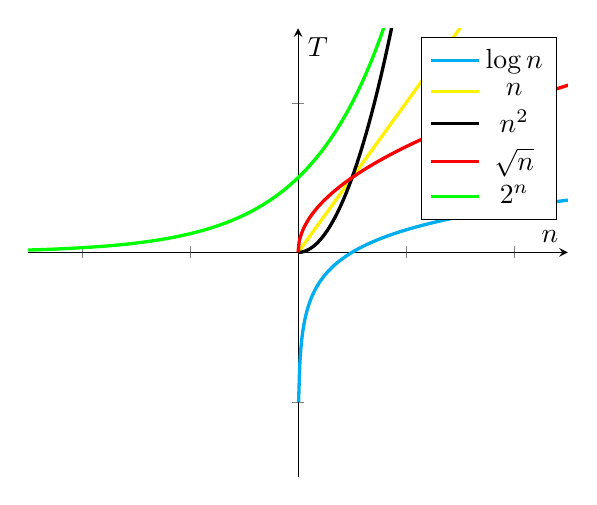
\begin{tikzpicture}
    \begin{axis}[xmin=-5,xmax=5,ymin=-3,ymax=3,axis x line=middle, axis y line=middle, yticklabel=\empty, xticklabel=\empty, xlabel=$n$, ylabel=$T$]
    \addplot [very thick,domain=-5:5,samples=500,color=cyan,]{log10(x)};\addlegendentry{$\log n$}
    \addplot [very thick,domain=0:10,samples=500,color=yellow,]{x};\addlegendentry{$n$}
    \addplot [very thick,domain=0:10,samples=500,color=black,]{x^2};\addlegendentry{$n^2$}
    \addplot [very thick,domain=0:10,samples=500,color=red,]{sqrt(\x)};\addlegendentry{$\sqrt{n}$}
    \addplot [very thick,domain=-5:5,samples=500,color=green,]{2^x};\addlegendentry{$2^n$}
    \end{axis}
\end{tikzpicture}

In informatica il calcolo asintotico è utilizzato per analizzare la complessità di un algoritmo. In particolar modo, per stimare quanto aumenta il tempo al crescere della dimensione n dell'input. Ma negli algoritmi non viene calcolata la costante del tempo, c'è bisogno di astrarre.

Esistono tre notazioni asintotiche:
\begin{itemize}
    \item Notazione asintotica $O$. \textit{O grande} è il limite superiore asintotico;
    \item Notazione asintotica $\Omega$. \textit{Omega} è il limite inferiore asintotico;
    \item Notazione asintotica $\Theta$. \textit{Theta} è il limite asintotico stretto.
\end{itemize}


\section{O grande}
L'O di una funzione, $O(g(n))$, è un'insieme di funzioni:
\begin{equation*}
    O(g(n))=\{f(n)|\exists c,n_0, c>0, n_0\geq0 \text{ t.c. } \forall n\geq n_0, f(n)\leq cg(n)\}
\end{equation*}

Ovvero rappresenta l'insieme di tutte le funzioni tali che devono essere dominate da $cg(n)$.
Ad esempio $O(n)$ rappresenta tutte le funzioni che sono dominate da $n$.

Stando a quanto detto $5n+38\in O(n)$ perchè $5n+38\leq5n+38n=43n\leq cn$. Infatti la funzione è dominata da $cn$ con $c$ almeno $43$ ed $n\geq1$. Si dice quindi che l'algoritmo assume la crescita di $n$ perchè posso astrarre dalle costanti moltiplicative e additive.

Con qualche passaggio in più possiamo applicare lo stesso discorso per i polinomi di grado d.
Ad esempio da $6n^3-2n+5$ derivano $c_3=6, c_2=0, c_1=2, c_0=5$.
\begin{equation*}
    \sum^d_{i=0}c_in^i=O(n^d)
\end{equation*}

Infatti $6n^3-2n+5\leq6n^3+5\leq6n^3+5n^3=11n^3\leq cn^3$ con $c\geq11$ e $n\geq1$.

Se invece voglio dimostrare che $\log_4n=O(\log_2n)$ dico che $\log_4n\leq c\log_2n$ ed effettuo un cambio di base:
$\log_bn=\frac{1}{\log_ab}*\log_an=cg(n)$. Notiamo come nei logaritmi non è importante la base, a tal punto che si indica solamente $O(\log)$.

Come classe di tutte le costanti, infine, si prende sempre la classe 1. Ad esempio $50\in O(1)$.

Se ho due funzioni e voglio sapre se $f(n)=O(g(n))$ posso calcolare il $\lim_{n\to+\infty}\frac{f(n)}{g(n)}$. Affinchè sia vero che $f(n)=O(g(n))$ \underline{non} devo ottenere $+\infty$, in tutti gli altri casi la funzione è dominata da $O(g(n))$.

\section{Omega}
L'Omega è sostanzialmente l'opposto dell'O grande. Intuitivamente con l'Omega dico che la complessità cresce almeno quanto ... ovvero non scende sotto a quel valore.
\begin{equation*}
     \Omega(g(n))=\{f(n)|\exists c,n_0, c>0, n_0\geq0 \text{ t.c. } \forall n\geq n_0, f(n)\geq cg(n)\}
\end{equation*}
Ovvero in $\Omega(g(n))$ troviamo tutte le funzioni che dominano la funzione $g(n)$.
Anche con $\Omega$ posso astrarre dalle constati moltiplicative e additive e applicare i metodi visti precedentemente.

\section{Theta}

Quando O e Omega coincidono otteniamo Theta. Diciamo quindi che la complessità è esattamente dell'ordine $\Theta(...)$ e per calcolarla 
è necessario che $O$ e $\Omega$ coincidono, ovvero che il loro limite sia finito.
\begin{equation*}
    \Theta(g(n)) = \{f(n)| \exists c_1>0,c_2>0,n_0\geq0 \text {t.c. } c_2*g(n)\leq f(n)\leq c_1*g(n),\forall n \geq n_0\}
\end{equation*}
\begin{equation*}
    \Theta(g(n)) = O(g(n)) \cap \Omega(g(n))
\end{equation*}
\begin{example}
    \begin{equation*}
        \sum^n_{i=1}i=\frac{n(n+1)}{2}
    \end{equation*}
    \begin{itemize}
        \item[-] $O(n^2)$ perchè $\frac{n(n+1)}{2}\leq cn^2$
        \item[-] $\Omega(n^2)$ perchè $\frac{n(n+1)}{2}\geq cn^2$
        \item[-] $\Theta(n^2)$ perchè $O(n^2)=\Omega(n^2)$
    \end{itemize}
    
    In altro modo, direttamente con la sommatoria, vedo che:
    \begin{itemize}
        \item[-] $\sum i=O(n^2)$ perchè $\sum^n_{i=1}i\leq\sum n=n^2=cn^2$
        \item[-] $\sum i=\Omega(n^2)$ perchè $\sum^n_{i=1}=1+2+3+...+\frac{n}{2}+...+n\geq\frac{n}{2}(\frac{n}{2}+1)+...+n\geq(\frac{n}{2})\frac{n}{2}$ volte $=\frac{n}{2}\frac{n}{2}=\frac{n^2}{4}=cn^2$
        \item[-] $\Theta(n^2)$ perchè $O(n^2)=\Omega(n^2)$
    \end{itemize}
\end{example}

\chapter{Sommatorie}
\section{Sommatorie algebriche}
Le sommatorie algebriche sono del tipo $\sum^n_{i=1}i=\frac{n(n+1)}{2}=\Theta(n^2)$. A noi interessa il valore di grandezza quindi a volte è inutile calcolarle in maniera esplicita. Ad esempio:
\begin{equation*}
    \sum^n_{i=1}i^c=\Theta(n^{c+1})\hspace{1cm}\sum^n_{i=1}i^3=\Theta(n^4)
\end{equation*}

\section{Sommatorie geometriche}
\begin{itemize}
    \item \begin{equation*}\sum^n_{i=0}c^i=\frac{c^{n+1}-1}{c-1}\end{equation*}$$\forall c\begin{cases}\Theta(c^n)\hspace{0.5cm}c>1\\\Theta(n)\hspace{0.5cm}c=1\\\Theta(1)\hspace{0.5cm}c<1\end{cases}$$
    
    \item \begin{equation*}\sum^n_{i=1}ic^i\approx\Theta(nc^n)\hspace{1cm}\sum^n_{i=1}i2^i\approx\Theta(n2^n)\end{equation*}
    \item \begin{equation*}\sum^n_{i=1}\log_2i\approx\Theta(n\log n)\end{equation*}
\end{itemize}

\section{Sommatorie armoniche}
\begin{itemize}
    \item \begin{equation*}\sum^n_{i=1}\frac{1}{i}\approx\int_1^n\frac{1}{x}dx=\left[\log_ex\right]_1^n=\Theta(\log n)\end{equation*}
\end{itemize}


\chapter*{Esercizi svolti}
\addcontentsline{toc}{chapter}{Esercizi svolti}
\begin{exercise}
    Calcolare il costo computazionale del seguente algoritmo:
    \begin{lstlisting}[language=Python]
        def es1(n):
            if n<0: n=-n
            while n!=0:
                if n%2: return 1
                n -= 2
            return 0
    \end{lstlisting}
    
    In questo esercizio notiamo che se n è dispari la complessità è O(1), se è pari O(n). Ne deduciamo che O(n) domina la complessità perchè l'algoritmo non farà mai peggio di O(n).
\end{exercise}

\begin{exercise}
    Calcolare il costo computazionale del seguente algoritmo:
    \begin{lstlisting}[language=Python]
        def es2(n):
            n=abs(n)
            x=z=0
            while x*x<n:
                x+=1
                z+=3x
            return z
    \end{lstlisting}
    
    Il ciclo while viene eseguito $\sqrt{n}$ volte. La complessità è dell'ordine $\sqrt{n}$ e in particolar modo $O(\sqrt{n})$, $\Omega(\sqrt{n})$, quindi $\Theta(\sqrt{n})$.
    
\end{exercise}

\begin{exercise}
    Calcolare il costo computazionale del seguente algoritmo:
    \begin{lstlisting}[language=Python]
        def es3(n):
            n=abs(n)
            x=z=0
            while n>1:
                r+=2
                n=n//3
            return z
    \end{lstlisting}
    
    La complessità è $\Theta(\log(n))$ perchè il ciclo while viene eseguito $\frac{n}{3^i}$ volte, fino a quando $n=1$. Quindi $\frac{n}{3^i}\approx1$, $n\approx3^i$, $\log_3n\approx\log_3^i$.
    
\end{exercise}

\begin{exercise}
    Calcolare il costo computazionale del seguente algoritmo:
    \begin{lstlisting}[language=Python]
        def es4(n):
            n=abs(n)
            t=x=1
            for i in range(n):
                t=3*t
            while t>x:
                x+=2
                t=t-2
            return z
    \end{lstlisting}
    
    La comlessità del for è $\Theta(n)$. Dopo il for $t=3^n$. Nel while t, dopo i primi passi, diventa $3^n-2i$, mentre $x=2i+1$. Otteniamo così $3^n-2i\approx2i+1=3^n\approx4i$, con $i=\frac{3^n}{4}=\Theta(3^n)$.
\end{exercise}

\begin{exercise}
    Calcolare il costo computazionale del seguente algoritmo:
    \begin{lstlisting}[language=Python]
        def es6(n):
            n=abs(n)
            u=t=s=1
            while u<=n:
                for j in range(t):
                    s+=1 
                u+=1
                t+=1
            return s
    \end{lstlisting}
    
    Il ciclo while viene eseguito $n+1$ volte, mentre il for $\sum^n_{i=1}\Theta(i)=\Theta(\sum^n_{i=1})=\Theta(n^2)$ che è la complessità dell'algoritmo.
\end{exercise}

\begin{exercise}
    Calcolare il costo computazionale del seguente algoritmo:
    \begin{lstlisting}[language=Python]
        def es7(n):
            n=abs(n)
            s=t=n
            p=0
            while s>=1:
                s=s//4
                p+=1
            while n>p:
                n-=p
                t+=5
            return t
    \end{lstlisting}
    
    Il primo ciclo while viene eseguito $\log_4(n)$ volte. Il secondo while viene eseguito $n-i\log(n)\approx0$ ovvero $i=\frac{n}{\log(n)}$. Il programma ha complessità $\Theta(\frac{n}{\log(n)})$.
\end{exercise}

\begin{exercise}
    Calcolare il costo computazionale del seguente algoritmo:
    \begin{lstlisting}[language=Python]
        def es8(n):
            n=abs(n)
            s=n
            p=2
            i=r=1
            while s>=1:
                s=s//5
                p+=2
            p=p*p
            while i*i*i>n:
                for j in range(p):
                    r+=1
                i+=1
            return r
    \end{lstlisting}
    
    Il primo while viene eseguito $\Theta(\log(n))$ volte. Il secondo while viene eserguito $i^3\approx n$ quindi $i=\sqrt[3]{n}$. Il for viene eserguito $\log^2(n)$ volte. Essendo il for dentro il while la complessità totale risulta essere $\Theta(\sqrt[3]{n}\log^2(n))$.
\end{exercise}

\begin{exercise}
    Calcolare il costo computazionale del seguente algoritmo:
    \begin{lstlisting}[language=Python]
        def es9(n):
            tot=n
            if n<=100: return s
            j=512
            while j>=2:
                k=1
                while k*k<=n:
                    k=2*k
                tot=tot+5
                j=j//2
            return t*t
    \end{lstlisting}
    
    Il primo while viene eseguito $\Theta(1)$ volte, perchè $j$ è settato ad una costante: 512. Il secondo while viene eseguito $2^i*2^i\approx n=2^2i\approx n$. Il programma ha complessità totale $\Theta(\log(n))$.
\end{exercise}

\begin{exercise}
    Calcolare il costo computazionale del seguente algoritmo:
    \begin{lstlisting}[language=Python]
        def es10(n):
            n=abs(n)
            p=2
            while n>=p:
                p=p*p
            return p
    \end{lstlisting}
    
    Il primo while viene eseguito $i=p^2,p^4,p^8,p^{2^i}$ quindi $2^{2^i}\approx n$ vuol dire che il programma ha complessità $\Theta(\log(\log(n)))$.
\end{exercise}

